\section{Auswertung}
\label{sec:Auswertung}
\subsection{Bestimmung der Brennweite über Gegenstands- und Bildweite.}
Zur Bestimmung der Brennweiten wird die Gleichung \eqref{eqn:LG} verwendent.
Die so erhaltenen Brennweiten werden gemittel. Daraus ergibt, dass die bestimmte
mittlere Brennweite $ \bar{f_{L}}$ für die Linse mit einer Brennweite von \SI{100}{\milli\meter}
\begin{equation*}
  \bar{f_{L}} = \SI{0.0983(4)}{\meter}
\end{equation*}
beträgt. Für die mittlere Brennweite der Wasserlinse $ \bar{f_{W}}$ ergibt
sich
\begin{equation*}
  \bar{f_{W}} = \SI{0.076(2)}{\meter} \; .
\end{equation*}
Die Darstellungen in Abbildung \ref{fig:gb} zeigen beide bei den entsprechen
den Werten für die jeweiligen Brennweiten einen ungefähren Häufungspunkt.
Der Abbildungsmaßstab wurde mit der Gleichung \eqref{eqn:AG} einmal mit
den Gegenstands- und Bildweiten und einmal mit den Gegenstands- und Bildgrößen
berechnet. Die so erhaltenen Abbildungsmaßstäbe wurden gemittel.
Die Gegenstandsgröße $G$ beträgt \SI{3}{\centi\meter}.
Dann ergbit sich für den mittleren Abbildungsmaßstab bestimmt über die
Gegenstands- und Bildweiten
\begin{equation*}
  \bar{V_{gb}} = \SI{1.5(6)}{}
\end{equation*}
und für den mittleren Abbildungsmaßstab bestimmt über die Gegenstands- und Bildgrößen
\begin{equation*}
  \bar{V_{GB}} = \SI{1.4(6)} \; .
\end{equation*}

\begin{figure}
  \centering
    \begin{subfigure}{0.48\textwidth}
      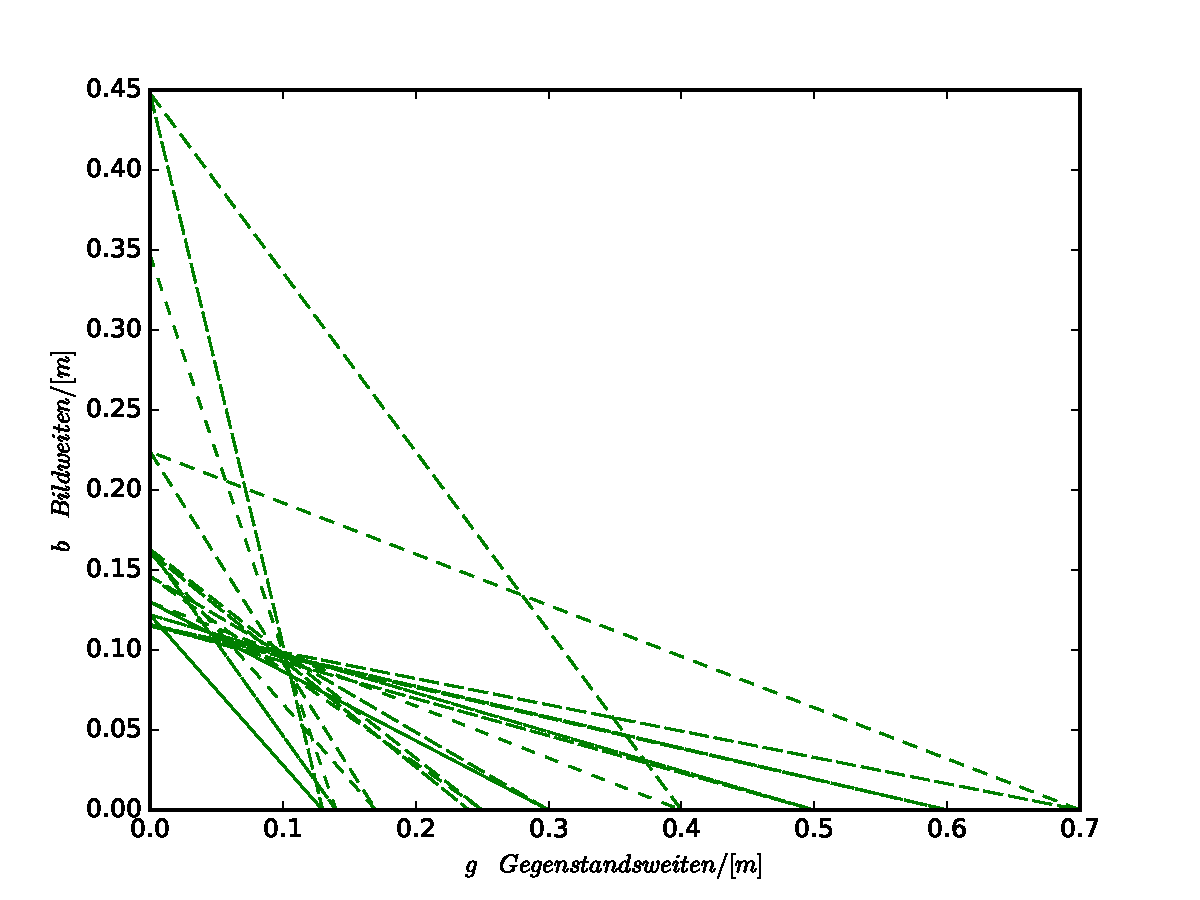
\includegraphics[height = 6cm]{plots/100mmLinsegbplot.pdf}
      \caption{Die Wertepaare \texorpdfstring{$\left(g_i , b_i \right)$}{math}
       für die Linse mit einer Brennweite von 100mm wurden in diesem
       Koordinatensystem eingetragen und durch eine Gerade verbunden. }
      \label{fig:Lgb}
    \end{subfigure}
    \begin{subfigure}{0.48\textwidth}
      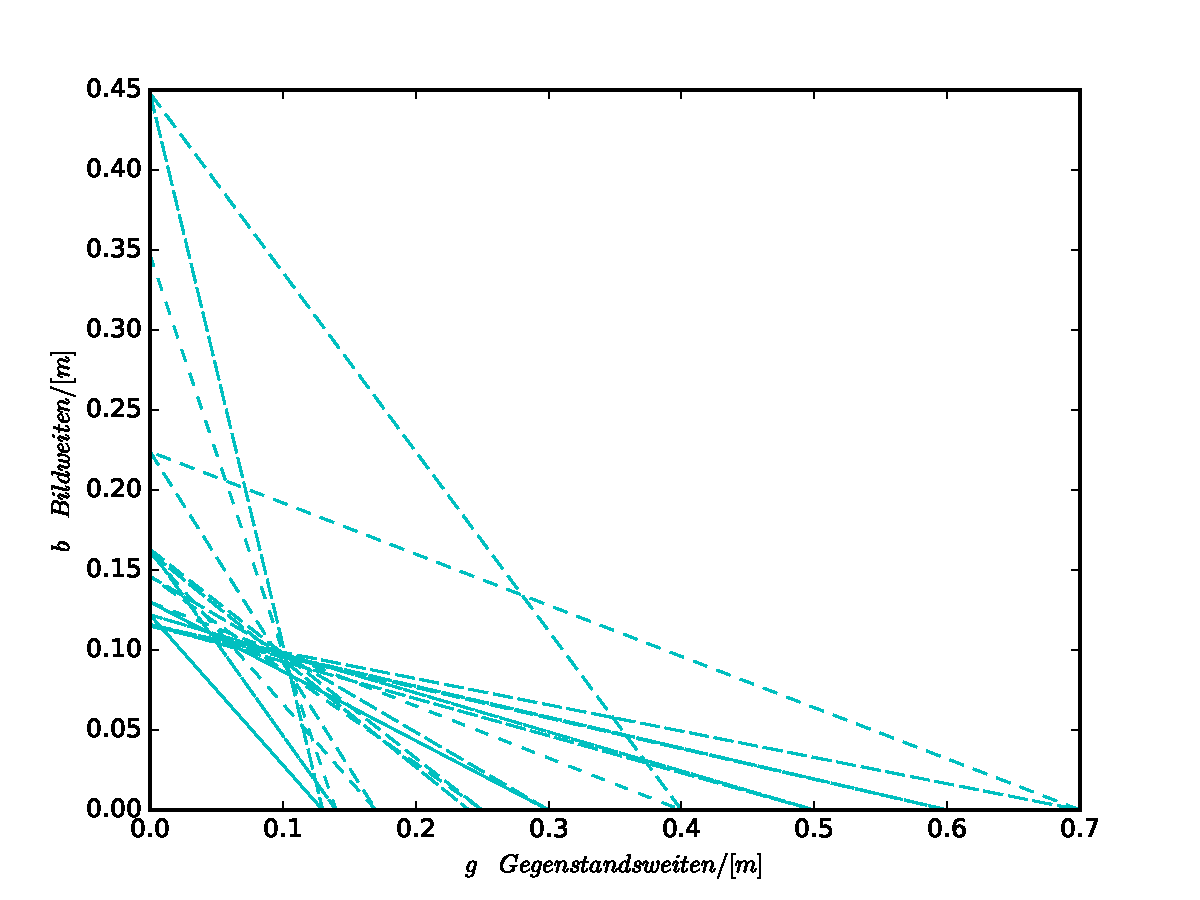
\includegraphics[height = 6cm]{plots/Wasserlinsegbplot.pdf}
      \caption{Die Wertepaare \texorpdfstring{$\left(g_i , b_i \right)$}{math}
       für die Wasserlinse wurden in diesem Koordinatensystem eingetragen und durch eine Gerade verbunden. }
      \label{fig:Wgb}
    \end{subfigure}
    \caption{Darstellungen zur Bestimmung der Brennweite über Gegenstands- und Bildweite.}
    \label{fig:gb}
\end{figure}
\FloatBarrier

\begin{table}
  \centering
  \sisetup{round-mode = places , round-precision = 2, scientific-notation = fixed, fixed-exponent=0}
  \begin{tabular}{S[round-precision = 0] S[round-precision = 0] S }
    \toprule
    $\text{g} / \si{\milli\meter}$ &
     $\text{b}/\si{\milli\meter} $ & $\text{f}_L / \si{\milli\meter}$\\
    \midrule
    1.400000000000001137e+02 & 3.470000000000000000e+02 & 9.975359342915818672e+01\\
    2.500000000000001137e+02 & 1.630000000000000284e+02 & 9.866828087167073136e+01\\
    2.999999999999999432e+02 & 1.459999999999999147e+02 & 9.820627802690577823e+01\\
    3.999999999999998863e+02 & 1.300000000000000000e+02 & 9.811320754716982151e+01\\
    1.299999999999998863e+02 & 4.480000000000000568e+02 & 1.007612456747404224e+02\\
    4.999999999999998863e+02 & 1.220000000000001137e+02 & 9.807073954983930264e+01\\
    6.000000000000000000e+02 & 1.159999999999999858e+02 & 9.720670391061452165e+01\\
    7.000000000000000000e+02 & 1.149999999999999858e+02 & 9.877300613496930737e+01\\
    1.699999999999999432e+02 & 2.240000000000000853e+02 & 9.664974619289338875e+01\\
    2.400000000000000000e+02 & 1.610000000000001421e+02 & 9.635910224438907790e+01\\
    \bottomrule
  \end{tabular}
  \caption{Werte der Gegenstadsweiten (g), der Bildweite (b)
  und der Brennweite (f) für die Linse mit Brennweite 100mm. }
  \label{tab:Lgb}
\end{table}
\begin{table}
  \centering
  \sisetup{round-mode = places , round-precision = 2, scientific-notation = fixed, fixed-exponent=0}
  % \resizebox{\textwidth}{!}{
  \begin{tabular}{S[round-precision = 0] S[round-precision = 0] S}
    \toprule
    $\text{g} / \si{\milli\meter}$ &
     $\text{b}/\si{\milli\meter} $ & $\text{f}_W / \si{\milli\meter} $\\
    \midrule
      8.299999999999995737e+01 & 2.060000000000000853e+02 & 5.916262975778545297e+01\\
      1.899999999999999432e+02 & 1.280000000000000000e+02 & 7.647798742138364503e+01\\
      2.400000000000000000e+02 & 1.159999999999998863e+02 & 7.820224719101116762e+01\\
      3.099999999999999432e+02 & 1.020000000000000853e+02 & 7.674757281553402777e+01\\
      2.900000000000000568e+02 & 1.059999999999998721e+02 & 7.762626262626255880e+01\\
      2.099999999999999716e+02 & 1.240000000000001137e+02 & 7.796407185628746106e+01\\
      1.499999999999999147e+02 & 1.600000000000000284e+02 & 7.741935483870965129e+01\\
      1.299999999999998863e+02 & 1.950000000000000568e+02 & 7.799999999999997158e+01\\
      1.099999999999998721e+02 & 2.620000000000001137e+02 & 7.747311827956984587e+01\\
      2.700000000000000000e+02 & 1.139999999999999858e+02 & 8.015625000000000000e+01\\
    \bottomrule
  \end{tabular}
  % }
  \caption{Werte der Gegenstadsweiten (g), der Bildweite (b)
  und der Brennweite (f), für die Wasserlinse.}
  \label{tab:Wgb}
\end{table}
\begin{table}
  \centering
  \sisetup{round-mode = places , round-precision = 2, scientific-notation = fixed, fixed-exponent=0}
  \begin{tabular}{S[round-precision = 0] S[round-precision = 0] S }
    \toprule
    $\text{g} / \si{\milli\meter}$ &
     $\text{b}/\si{\milli\meter} $ & $\text{B} / \si{\milli\meter} $\\
    \midrule
    1.400000000000001137e+02 & 3.470000000000000000e+02 & 7.200000000000001421e+01\\
    2.500000000000001137e+02 & 1.630000000000000284e+02 & 1.900000000000000000e+01\\
    2.999999999999999432e+02 & 1.459999999999999147e+02 & 1.399999999999999822e+01\\
    3.999999999999998863e+02 & 1.300000000000000000e+02 & 1.000000000000000000e+01\\
    1.299999999999998863e+02 & 4.480000000000000568e+02 & 1.000000000000000000e+02\\
    \bottomrule
  \end{tabular}
 \caption{Werte der Gegenstadsweiten (g) und der Bildweite (b)
  und B ist die Bildgröße für die Linse mit Brennweite 100mm.}
  \label{tab:Bgb}
\end{table}

\FloatBarrier
\subsection{Bestimmung der Brennweite nach der Methode von Bessel.}
Die Brennweiten werden nach der Fromel \eqref{eqn:bessel} bestimmt und
gemittelt. Dann ergibt sich für die mittlere Brennweite für weißes Licht
\begin{equation*}
  \bar{f_n} = \SI{0.0988(5)}{\meter}
\end{equation*}
und  für die mittlere Brennweite für rotes $\bar{f_r}$ und blaues
$\bar{f_b}$ Licht
\begin{equation*}
  \bar{f_r} = \SI{0.0999(5)}{\meter} \qquad  \bar{f_b} = \SI{0.0992(8)}{\meter} \; .
\end{equation*}
Alle Werte dazu sind in den Tabellen \ref{tab:bn} , \ref{tab:bb} und \ref{tab:br}
dargestellt. Fest zuhalten ist, dass die Brennweiten für rotes und blaues Licht
größer sind als die für normales Licht. Auch hier wurde wieder mit einer Linse
mit einer Brennweite von \SI{100}{\milli\meter} gearbeitet.
\begin{table}
  \centering
  \sisetup{round-mode = places , round-precision = 0,scientific-notation=fixed, fixed-exponent = 0}
  % \resizebox{\textwidth}{!}{%
  \begin{tabular}{S S S }
    \toprule
    $\text{e}_n / \si{\milli\meter}$ &
     $\text{d}_n /\si{\milli\meter} $ & $\text{f}_n / \si{\milli\meter} $\\
    \midrule
    6.500000000000000000e+02 & 3.990000000000000568e+02 & 1.012688461538461269e+02\\
    6.000000000000000000e+02 & 3.490000000000001137e+02 & 9.924958333333330529e+01\\
    5.500000000000000000e+02 & 2.850000000000000568e+02 & 1.005795454545454675e+02\\
    5.000000000000000000e+02 & 2.200000000000000000e+02 & 1.007999999999999972e+02\\
    4.500000000000000000e+02 & 1.589999999999999147e+02 & 9.845500000000001251e+01\\
    4.000000000000000000e+02 & 4.699999999999988631e+01 & 9.861937500000001933e+01\\
    8.500000000000000000e+02 & 6.250000000000000000e+02 & 9.761029411764702957e+01\\
    8.000000000000000000e+02 & 5.740000000000000000e+02 & 9.703875000000005002e+01\\
    7.500000000000000000e+02 & 5.210000000000000000e+02 & 9.701966666666665162e+01\\
    7.000000000000001137e+02 & 4.650000000000000000e+02 & 9.777678571428575083e+01\\
    \bottomrule
  \end{tabular}
  % }
  \caption{Werte der Brennweite \texorpdfstring{$f_n$}{math}, berechnet aus
  \texorpdfstring{$e_n$}{math} der Abstand zwischen Schirm und Gegenstand und
  \texorpdfstring{$d_n$}{math} Abstand der Linsenpositionen für normales Licht.}
  \label{tab:bn}
\end{table}
\begin{table}
  \centering
  \sisetup{round-mode = places , round-precision = 0,scientific-notation=fixed, fixed-exponent = 0}
  % \resizebox{\textwidth}{!}{
  \begin{tabular}{S S S}
    \toprule
     $\text{e}_b / \si{\milli\meter}$ &
     $\text{d}_b /\si{\milli\meter} $ & $\text{f}_b / \si{\milli\meter} $\\
    \midrule
    7.000000000000001137e+02 & 4.559999999999999432e+02 & 1.007371428571428993e+02\\
    6.500000000000000000e+02 & 4.000000000000000000e+02 & 1.009615384615384670e+02\\
    6.000000000000000000e+02 & 3.480000000000000000e+02 & 9.954000000000000625e+01\\
    5.000000000000000000e+02 & 2.350000000000000284e+02 & 9.738749999999998863e+01\\
    4.000000000000000000e+02 & 6.400000000000005684e+01 & 9.743999999999999773e+01\\
    \bottomrule
  \end{tabular}
  % }
  \caption{Werte der Brennweite \texorpdfstring{$f_b$}{math}, berechnet aus
  \texorpdfstring{$e_b$}{math} der Abstand zwischen Schirm und Gegenstand und
  \texorpdfstring{$d_b$}{math} Abstand der Linsenpositionen für blaues Licht.}
  \label{tab:bb}
\end{table}
\begin{table}
  \centering
  \sisetup{round-mode = places , round-precision = 0,scientific-notation=fixed, fixed-exponent = 0}
  % \resizebox{\textwidth}{!}{
  \begin{tabular}{S S S S S S S}
    \toprule
      $\text{e}_r / \si{\milli\meter}$ &
     $\text{d}_r /\si{\milli\meter} $ & $\text{f}_r / \si{\milli\meter} $\\
    \midrule
    4.000000000000000000e+02 & 5.600000000000008527e+01 & 9.804000000000002046e+01\\
    5.000000000000000000e+02 & 2.260000000000000853e+02 & 9.946199999999997488e+01\\
    6.000000000000000000e+02 & 3.460000000000000000e+02 & 1.001183333333333394e+02\\
    6.500000000000000000e+02 & 4.009999999999999432e+02 & 1.006534615384615705e+02\\
    7.000000000000001137e+02 & 4.550000000000000000e+02 & 1.010625000000000284e+02\\
    \bottomrule
  \end{tabular}
  % }
  \caption{Werte der Brennweite \texorpdfstring{$f_r$}{math}, berechnet aus
  \texorpdfstring{$e_r$}{math} der Abstand zwischen Schirm und Gegenstand und
  \texorpdfstring{$d_r$}{math} Abstand der Linsenpositionen für rotes Licht.}
  \label{tab:br}
\end{table}




\FloatBarrier
\subsection{Bestimmung der Brennweite eines Linsensystems nach der Methode von Abbe.}
In den Diagrammen \ref{fig:gabbe} und \ref{fig:babbe} sind jeweils
$g'$ gegen $\left(1 + \frac{1}{V}\right)$ und $b'$ gegen $ \left(1 + V\; \right)$
aufgetragen. Wird nun durch Ausgleichsrechnung eine Gerade
\begin{equation*}
  f(x) = a \cdot x + b
\end{equation*}
durch die Messpunkte gelegt ergibt sich mit dem Zusammenhang \eqref{eqn:abbe}
\begin{equation*}
  a = f \qquad \text{und} \qquad b = h \qquad \text{bzw.} \qquad b = h' \; .
\end{equation*}
Daraus folgt für $g'$ :
\begin{equation*}
  f_{g'} = \SI{0.17(1)}{\meter} \qquad h = \SI{-0.04(5)}{\meter} \;.
\end{equation*}
Für $b'$ folgt:
\begin{equation*}
  f_{b'} = \SI{0.09(2)}{\meter} \qquad h' = \SI{0.24(2)}{\meter} \;.
\end{equation*}
\begin{figure}
  \centering
    \begin{subfigure}{0.48\textwidth}
      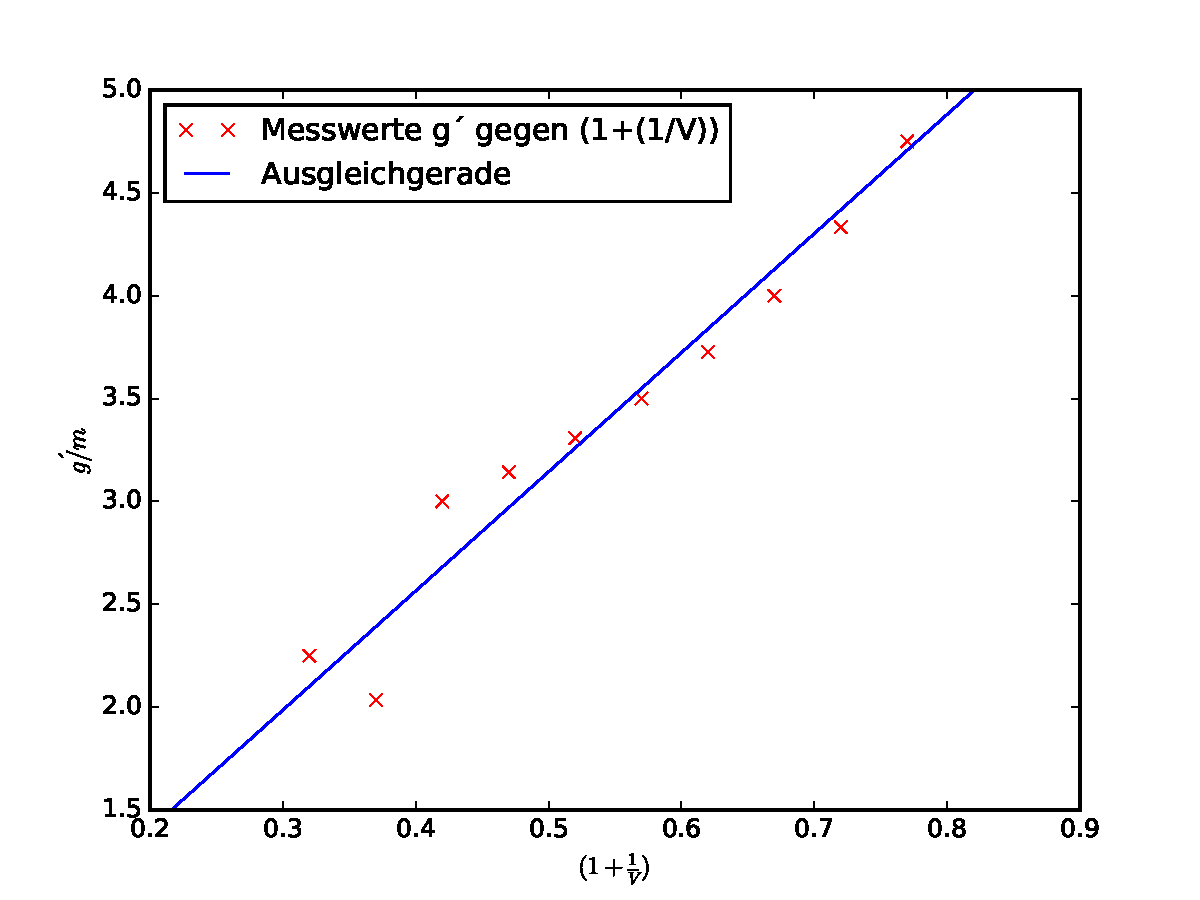
\includegraphics[height = 6cm]{plots/gsplot.pdf}
      \caption{In diesem Diagramm ist g' gegen
      \texorpdfstring{$\left(1 + \frac{1}{V}\right)$}{math} aufgetragen und
      eine Ausgleichgerade eingezeichnet. }
      \label{fig:gabbe}
    \end{subfigure}
    \begin{subfigure}{0.48\textwidth}
      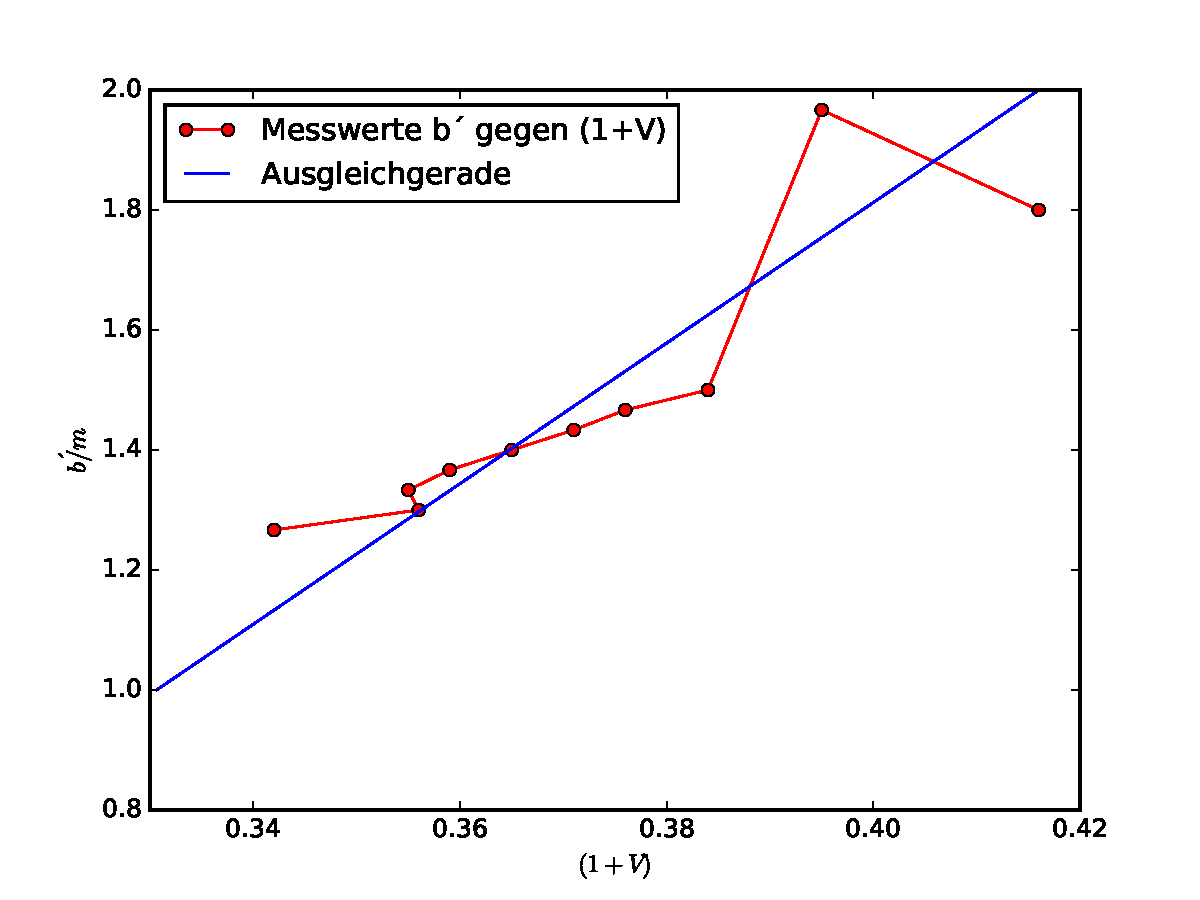
\includegraphics[height = 6cm]{plots/bsplot.pdf}
      \caption{In diesem Diagramm ist b' gegen (1 + V) aufgetragen und
      eine Ausgleichsgerade eingezeichnet. }
      \label{fig:babbe}
    \end{subfigure}
    \caption{Diagramme zur Bestimmung der Brennweite eines Linsensystems nach Abbe.}
    \label{fig:abbe}
\end{figure}
Alle Daten dazu sind in der Tabelle \ref{tab:abbe} dargestellt.
\begin{table}
  \centering
  \sisetup{round-mode = places , round-precision = 0,scientific-notation=fixed, fixed-exponent = 0}
  % \resizebox{\textwidth}{!}{%
  \begin{tabular}{S S S[round-precision=2] S[round-precision=2]}
    \toprule
    $\text{g'}/ \si{\milli\meter}$ &
    $\text{b'} /\si{\milli\meter}$ & ${1} {+}\frac{1}{V}$  & ${1} {+} V $\\
    \midrule
    3.200000000000000000e+02 & 4.160000000000000568e+02 & 2.250000000000000000e+00 & 1.799999999999999822e+00\\
    3.700000000000000000e+02 & 3.950000000000000000e+02 & 2.034482758620689502e+00 & 1.966666666666666785e+00\\
    4.200000000000000000e+02 & 3.840000000000000000e+02 & 3.000000000000000000e+00 & 1.500000000000000000e+00\\
    4.700000000000000568e+02 & 3.760000000000000000e+02 & 3.142857142857143238e+00 & 1.466666666666666563e+00\\
    5.200000000000000000e+02 & 3.710000000000000000e+02 & 3.307692307692307487e+00 & 1.433333333333333348e+00\\
    5.700000000000001137e+02 & 3.650000000000000000e+02 & 3.500000000000000000e+00 & 1.399999999999999911e+00\\
    6.200000000000000000e+02 & 3.590000000000000000e+02 & 3.727272727272727071e+00 & 1.366666666666666696e+00\\
    6.700000000000000000e+02 & 3.550000000000000000e+02 & 4.000000000000000000e+00 & 1.333333333333333259e+00\\
    7.200000000000000000e+02 & 3.560000000000000568e+02 & 4.333333333333333925e+00 & 1.300000000000000044e+00\\
    7.700000000000000000e+02 & 3.420000000000000000e+02 & 4.750000000000000000e+00 & 1.266666666666666607e+00\\
    \bottomrule
  \end{tabular}
  % }
  \caption{Werte zur Bestimmung der Brennweiten \texorpdfstring{$f_{g'}$}{math}
  und \texorpdfstring{$f_{b'}$}{math},
  g' ist der Abstand zwischen Gegenstand
  und Linsensystem und b' der Abstand zwischen Linsensystem und Schirm.
  V ist Abbildungsmaßstab.}
  \label{tab:abbe}
\end{table}
\FloatBarrier










%
